\documentclass[12pt]{amsart}

\usepackage{amsmath}
\usepackage{amssymb}
\usepackage{amsfonts}
\usepackage[alphabetic]{amsrefs}
\usepackage{amsthm}
\usepackage{enumitem}
\usepackage{fullpage}
\usepackage{color}
\usepackage{graphicx}
% \usepackage[parfill]{parskip}

\newcommand{\An}{\mathbb{A}^n}
\newcommand{\Pn}{\mathbb{P}^n}
\renewcommand{\a}{\mathfrak{a}}
\newcommand{\C}{\mathbb{C}}
\newcommand{\Z}{\mathbb{Z}}
\newcommand{\Q}{\mathbb{Q}}
\newcommand{\g}{\mathfrak{g}}
\newcommand{\h}{\mathfrak{h}}
\newcommand{\ad}{\mathrm{ad}}
\newcommand{\git}{/\!\!/}

\newtheorem*{theorem}{Theorem}
\newtheorem*{definition}{Definition}
\newtheorem*{corollary}{Corollary}
\newtheorem*{lemma}{Lemma}
\newtheorem*{exercise}{Exercise}
\newtheorem*{proposition}{Proposition}
\newtheorem*{claim}{Claim}
\newtheorem*{question}{Question}

\theoremstyle{remark}
\newtheorem*{remark}{Remark}

\theoremstyle{remark}
\newtheorem*{example}{Example}

\theoremstyle{remark}
\newtheorem*{moreexamples}{More examples}

\allowdisplaybreaks

\title{Root Systems Question}

\begin{document}
\maketitle

Let $\Phi$ be the root system of a complex semisimple Lie algebra.
The question is concerned with $|\Phi|$-tuples of nonnegative integers $\eta = (\eta_\alpha)_{\alpha\in\Phi} \in \left(\mathbb{Z}_{\ge 0}\right)^{|\Phi|}$.
We will call such a tuple $\eta \in \left(\mathbb{Z}_{\ge 0}\right)^{|\Phi|}$ an \emph{exponent}.

\begin{definition}
    An exponent $\eta \in (\Z_{\ge 0})^{|\Phi|}$ is \emph{admissible} if $\eta \ne 0$ and
    $$\sum_{\alpha \in \Phi} \eta_\alpha \alpha = 0.$$
\end{definition}

Observe that the sum of admissible exponents is admissible (here the sum of exponents is defined by regular addition of tuples of integers, i.e., $\eta+\nu = (\eta_\alpha+\nu_\alpha)_{\alpha\in\Phi}\in \left(\mathbb{Z}_{\ge 0}\right)^{|\Phi|}$).

\begin{question}
Can we find and describe a minimal set of admissible exponents so that any exponent can be expressed as a sum of exponents in the minimal set? 
\end{question}


\begin{definition}
For any exponent $\eta$, we can consider exponents $\tilde \eta = (\tilde \eta_\alpha)_{\alpha\in\Phi} \in (\Z_{\ge 0})^{|\Phi|}$ such that $0 \le \tilde \eta_\alpha \le \eta_\alpha$ for all $\alpha \in \Phi$, and the corresponding sum
$$\sum_{\alpha\in \alpha} \tilde \eta_\alpha \alpha,$$
which we call a \emph{subsum} of $\eta$.
Call an admissible exponent $\eta$ \emph{simple} if no nontrivial subsum of $\eta$ is zero.
\end{definition}

\begin{example}
    Consider the $A_1$ root system $\Phi=\{\alpha,-\alpha\}$.
    The exponent $\eta=(\eta_\alpha, \eta_{-\alpha}) = (1, 1)$ is admissible and simple.
    The exponent $\nu=(\nu_\alpha, \nu_{-\alpha}) = (2, 2)$ is admissible but not simple, since $\eta$ gives a subsum of $\nu$ which is zero.
\end{example}

It is straightforward to see that any admissible exponent is a sum of simple exponents.
Then the simple admissible exponents are the minimal generating set asked about in the question --- so our goal is to describe all simple admissible exponents.

Here is one way to find simple admissible exponents $\eta$:
choose positive roots $\Phi^+$ and let $\Delta$ be the corresponding simple roots;
pick any positive root $\beta \in \Phi$ and express it as a sum of simple roots $\beta=\sum_{\alpha\in\Delta} n_\alpha \alpha$;
then define an exponent $\eta \in (\Z_{\ge 0})^{|\Phi|}$ by
$$
\eta_\alpha = \begin{cases}
    1, & \text{if } \alpha = \beta, \\
    n_\alpha, & \text{if } \alpha \in - \Delta, \\
    0, & \text{otherwise.}
\end{cases}$$
The exponent $\eta=(\eta_\alpha)_{\alpha\in\Phi}$ is admissible by construction.
It is also simple: any nontrivial subsum of $\eta$ which contains $\beta$ will be a positive-integer combination of simple roots and any nontrivial subsum of $\eta$ not containing $\beta$ will be a negative-integer combination of simple roots, so there can be no nontrivial subsums which give zero.

\begin{claim}[\textcolor{red}{unproven}]
Any simple admissible exponent arises in the way described above, for some choice of positive roots $\Phi^+$ and some $\beta \in \Phi^+$.
\end{claim}

I don't know how to prove this claim, though here is how we could potentially prove this:
if $\eta$ is admissible and simple, show that there must be some $\alpha \in \Phi$ such that $\eta_\alpha=1$;
show that the rest of the roots $\beta\in\Phi\setminus\{\alpha\}$ such that $\eta_\beta\ne0$ form a set of simple roots.

\section*{Examples of simple admissible exponents}
In this section we will show some examples of admissible exponents that led to the above claim.
For rank 2 root systems, we can denote admissible exponents by drawing the roots with nonzero coefficient in red, scaled by the coefficient corresponding to that root.
For example, if $\Phi=A_2$ labelled with the following choice of simple roots $\{\alpha, \beta\}$:

\centerline{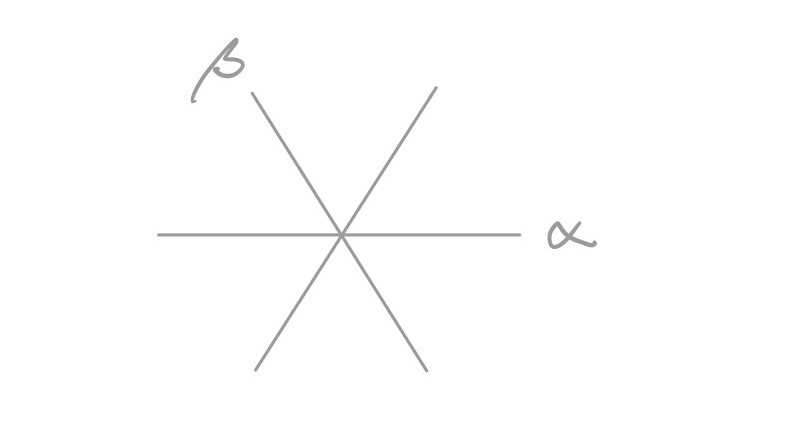
\includegraphics[scale=0.25]{A_2 root system.jpg}}

\noindent
We denote the admissible exponents $\eta, \nu$, where $\eta_{\alpha+\beta}, \eta_{-(\alpha+\beta)}=1$ and $\nu_{\alpha}, \nu_{-\alpha}=2$ and all other coefficients zero, by

\centerline{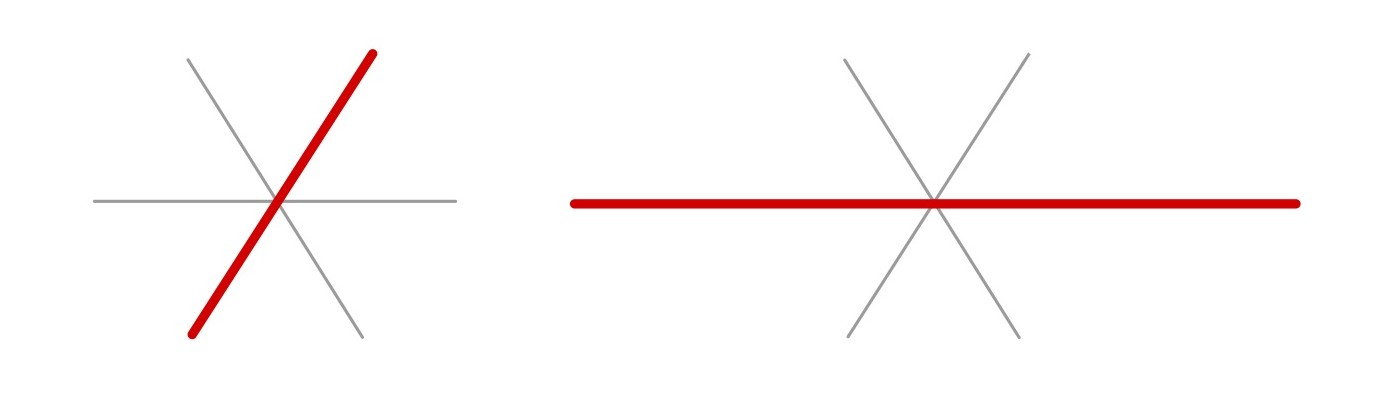
\includegraphics[scale=0.25]{A_2 diagram notation example.jpg}}

\noindent
We claim the following is the complete set of simple admissible exponents for $A_2$ (one can check these are all admissible and simple, but it is unclear whether this is a complete set):

\centerline{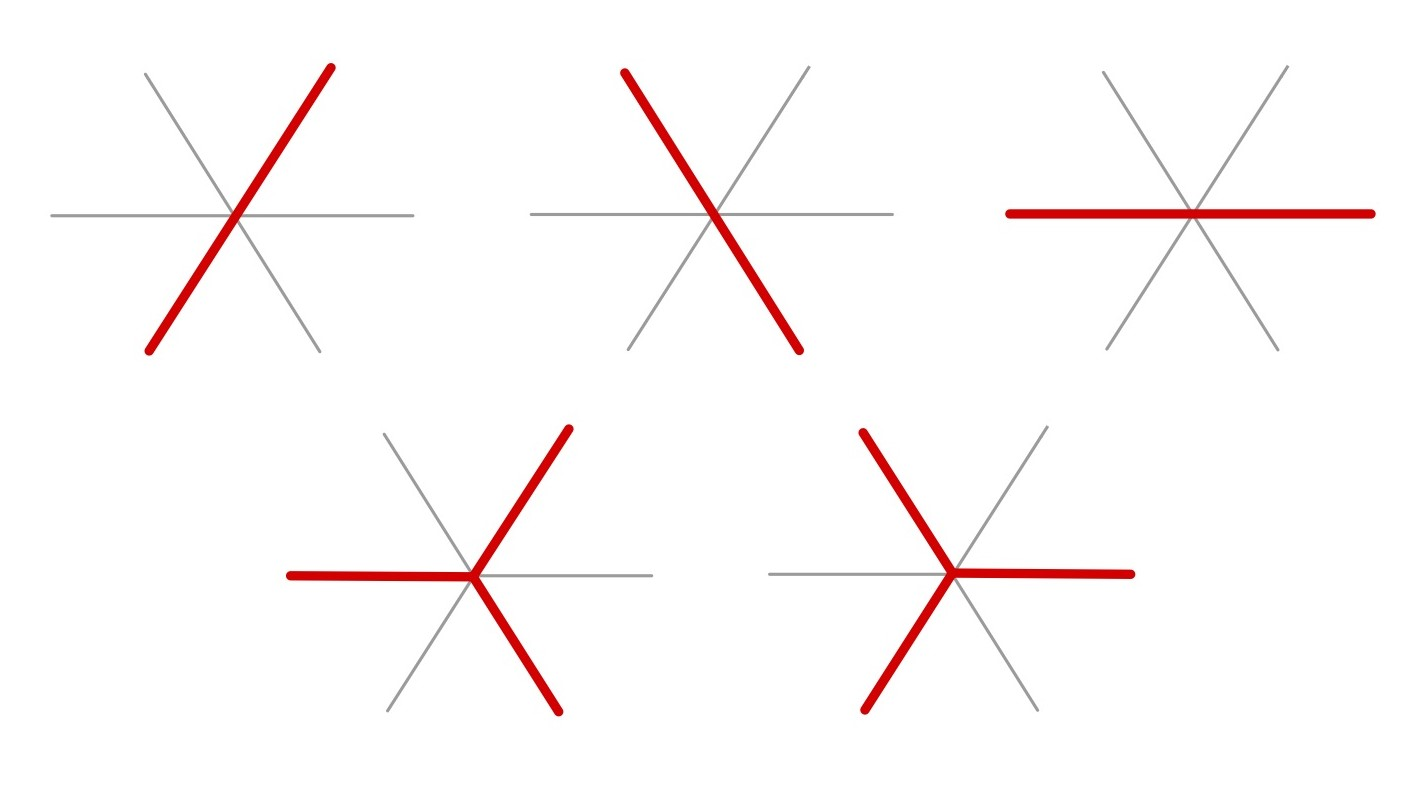
\includegraphics[scale=0.25]{A_2 simple admissibles.jpg}}

\newpage
\noindent
If we consider the $C_2$ root system with the following choice of simple roots

\centerline{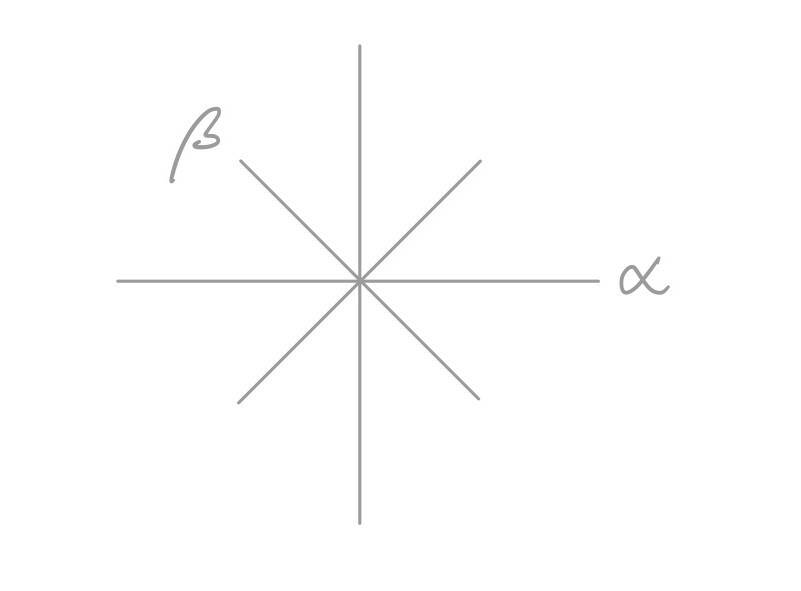
\includegraphics[scale=0.25]{C_2 root system.jpg}}

\noindent
Then we claim the following is the complete set of simple admissible exponents for $C_2$:

\centerline{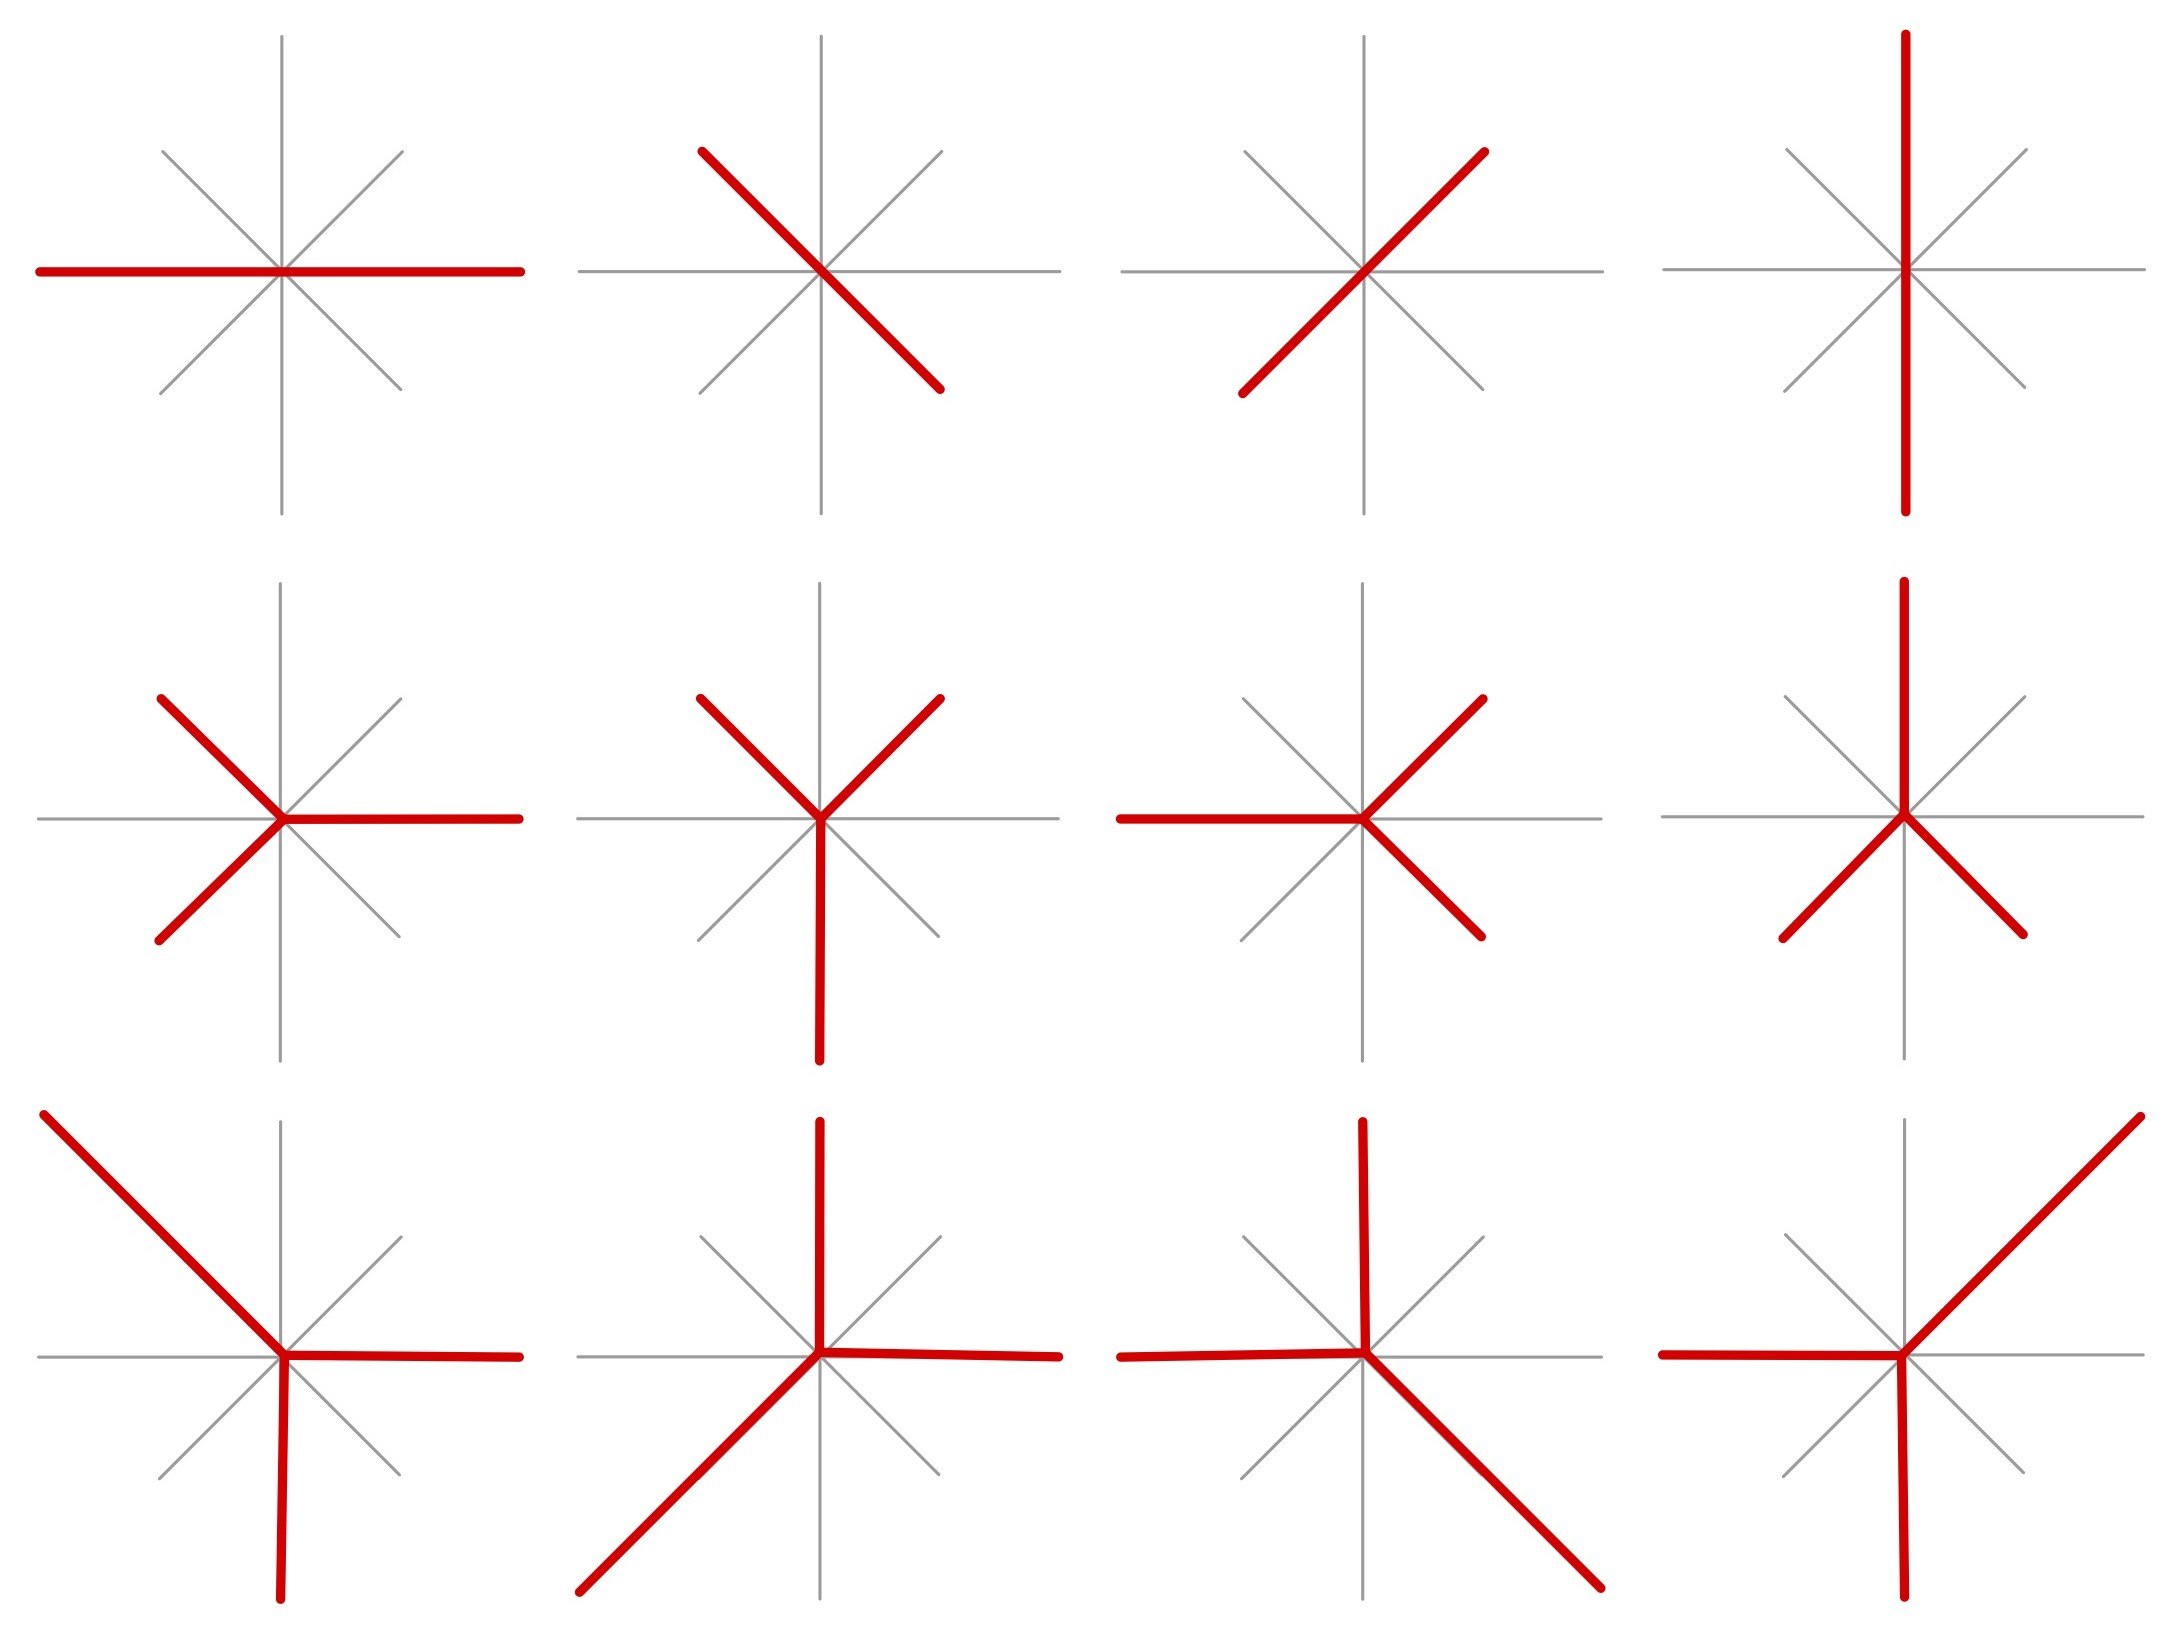
\includegraphics[scale=0.2]{C_2 simple admissibles.jpg}}

\end{document}